\documentclass[a4paper,11pt]{article}

\usepackage[utf8]{inputenc} \usepackage{mathpazo} \usepackage{gensymb}
\usepackage{graphicx} \usepackage{url} \usepackage[frenchb]{babel}
\usepackage{subfig} \usepackage{apacite} \usepackage{array}
\usepackage{multirow} \usepackage{dcolumn}
\newcolumntype{d}[1]{D{,}{,}{#1}} \usepackage[T1]{fontenc}
\usepackage{txfonts} \usepackage{amsmath} \usepackage{upgreek}
% \renewcommand{\thefootnote}{\Alph{footnote}}
% \usepackage[bottom]{footmisc}
% \usepackage{natbib} 
% \bibliographystyle{plainnat}
% \newcommand*{\dl}{\cline{2-2}\cline{4-4}}
% \usepackage [nottoc]{tocbibind}

\begin{document}

\title{De l' Extraction \& purification aux premières analyses de
  séquences d'ADN de sols du Burkina Faso} \author{Marilyne
  Aza-Gnandji} \date{\today}

\maketitle \tableofcontents
\newpage

\section{Du prélèvement d'échantillons de sols à l'extraction d'ADN}


\subsection{Prélèvement d'échantillons de sols}

Dans le cadre du projet Oracle(optimisation des systèmes de rotation
et d’associations de céréales et de légumineuses), des prélèvements de
sols représentatifs des parcelles agricoles ont été réalisés. Les
prélèvements ont été faits dans les zones de Yilou (20) , Sera (15),
Boussouma secteur2 (15), Tengressene (15), Raguitenga (15) soit 80
parcelles au total. Pour chaque parcelle, quatre coups de tarières ont
été mélangés à chaque angle d’un carré virtuel d’approximativement
deux mètres de côté. Pour chaque coup de tarière le sol superficiel a
été écarté à la truelle, et les 20 premiers centimètres ont été
prélevés. Les plus \og{}gros cailloux\fg{} ont été éliminés.  De
retour à Ouagadougou, les sols ont ensuite été laissés sécher à
température ambiante sur une paillasse au laboratoire, tamisés à 5 mm,
conditionnés et envoyés à Dakar. L'ADN environnemental par parcelle
d’étude a été réalisé (voir tableau~\ref{tableau:Nombre de parcelles
  échantillonnées par zone d'étude} et Fig.~\ref{fig-image1}
p.~\pageref{fig-image1}).  Par la suite, quatre extractions d'ADN
total par sol ont été réalisées, dont 2 extraits d’ADN conservés à
Dakar à -20\,\degree{}C et les 2 autres extraits d' ADN (lyophilisés)
ont été acheminés à Montpellier.


\begin{figure}
  \begin{center}
    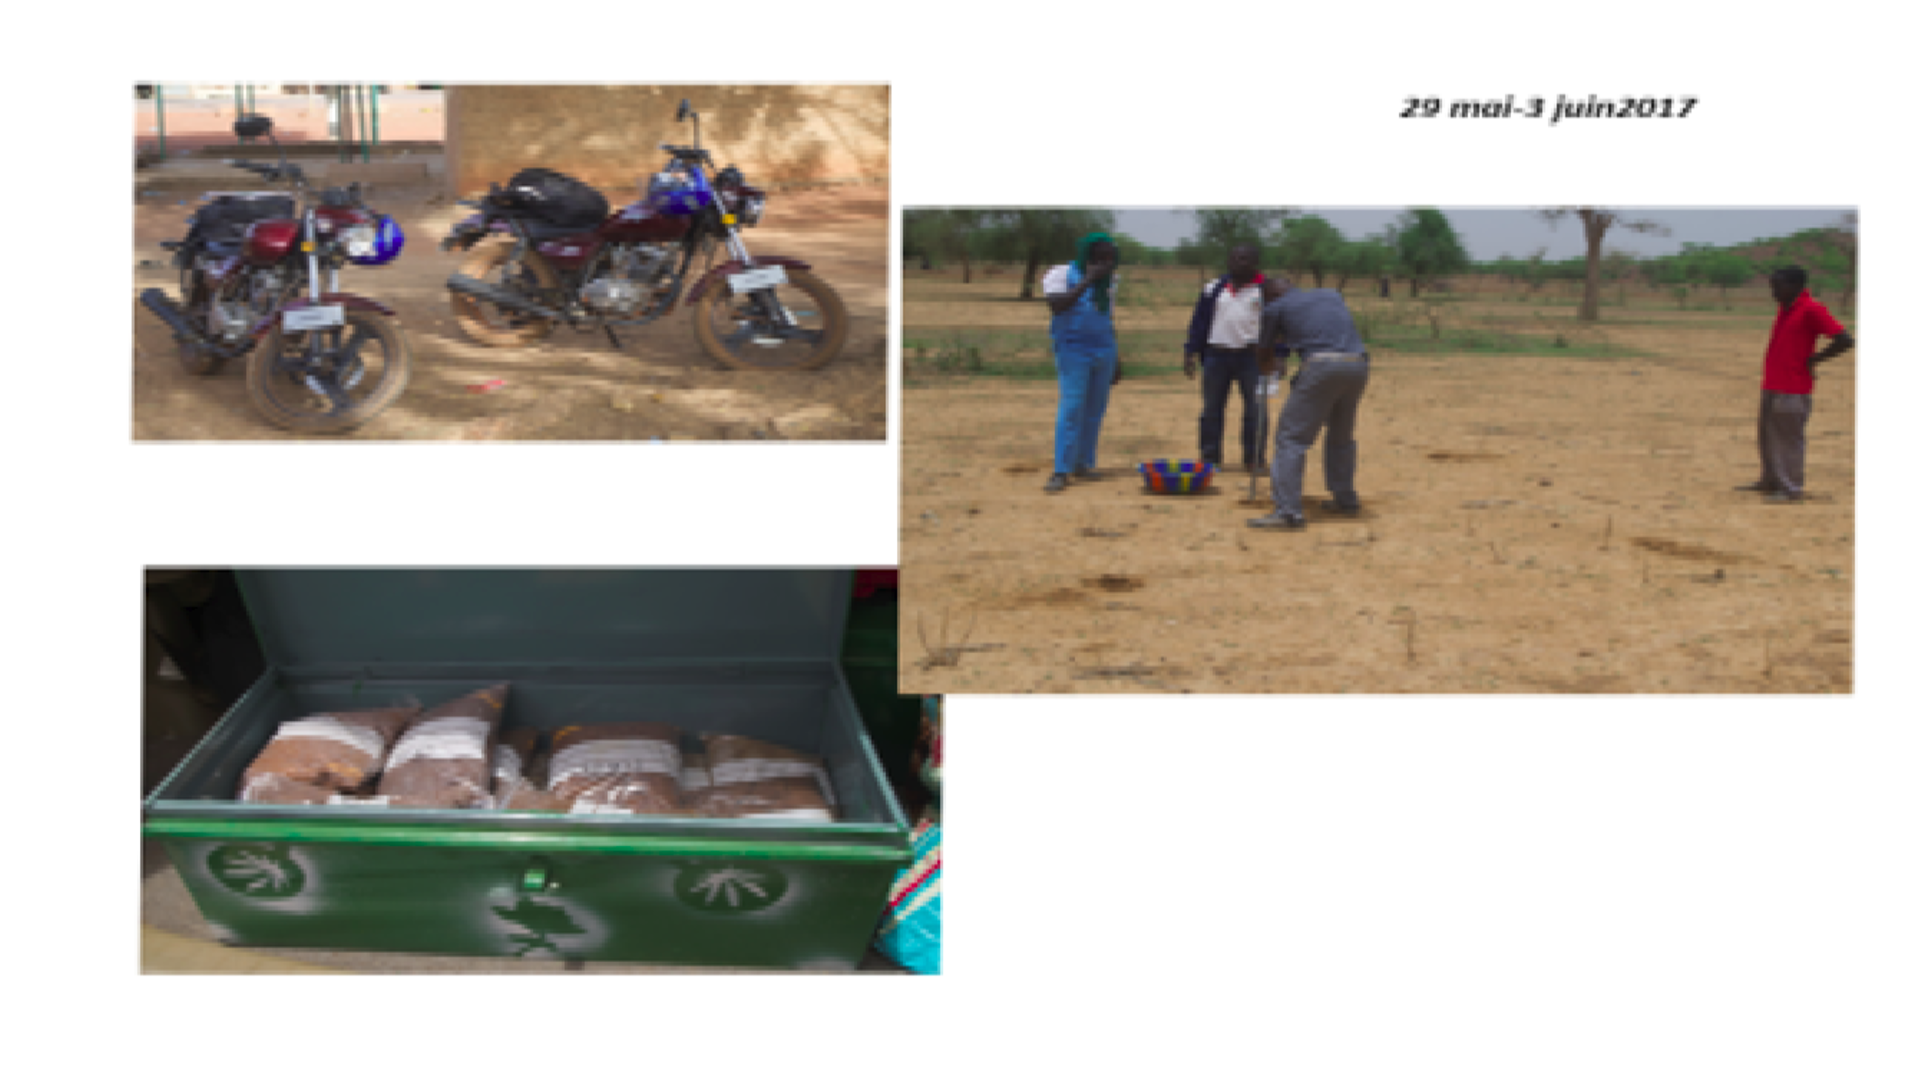
\includegraphics[width=16cm]{images/image1}
  \end{center}
  \caption{Etape de prélèvement des échantillons sur le terrain}
  \label{fig-image1}
\end{figure}

\begin{table}
  \begin{center}
    \begin{tabular}{|l|r|}
      \hline \multicolumn{1}{|c|}{Village}&\multicolumn{1}{c|}{Nombre
        de parcelles} \\ \hline Raguitenga & 15\\Boussouma secteur2 &
      15\\ Sera & 15 \\ Tengressene & 15\\ Yilou & 20\\ \hline
    \end{tabular}
    \caption{Nombre de parcelles échantillonnées par zone d'étude}
    \label{tableau:Nombre de parcelles échantillonnées par zone d'étude}
  \end{center}
\end{table}


\subsection{Extraction d'ADN}

Une première étape avant l'extraction est de peser une quantité de 500
mg par sol prélevé. Ensuite, un kit d'extraction d'ADN (FastDNA® Spin
Kit for soil) a été utilisé et le protocole du fournisseur a été
déroulé.

\begin{figure}
  \begin{center}
    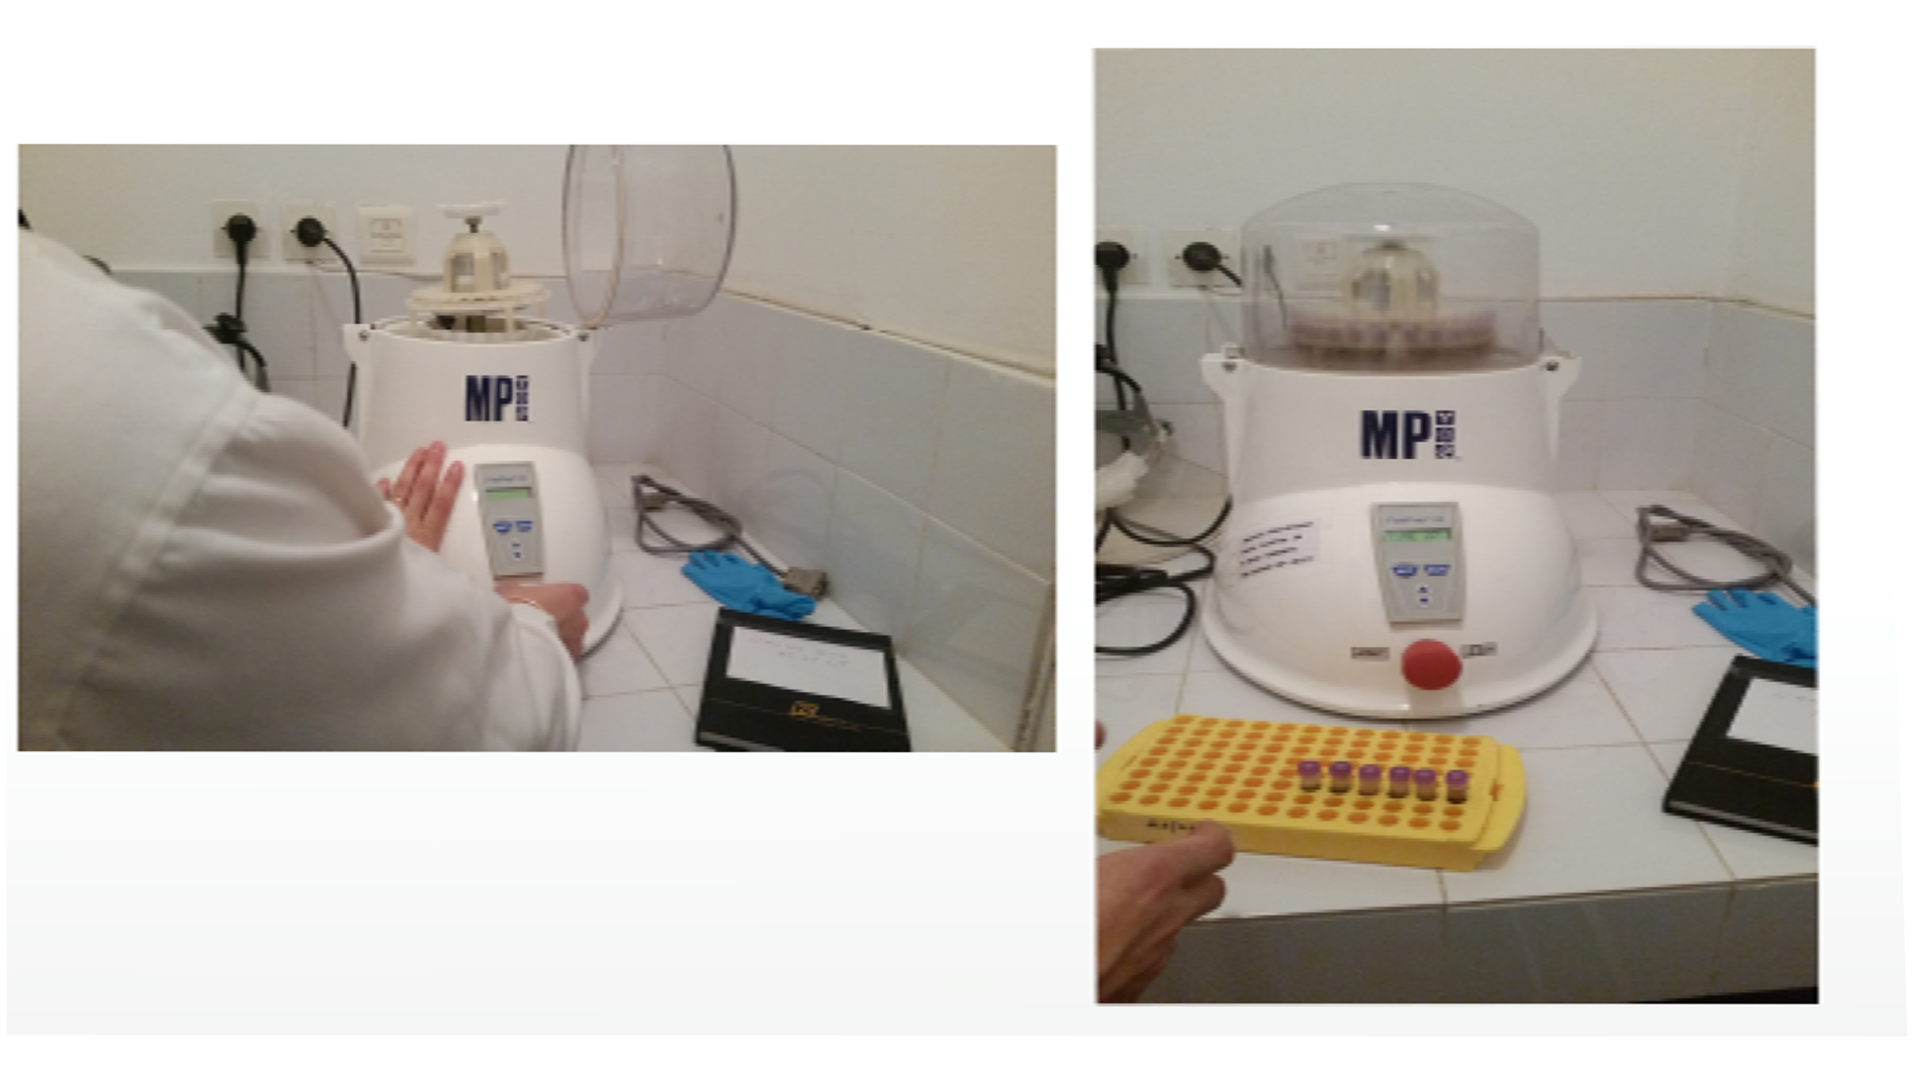
\includegraphics[width=16cm]{images/image2}
  \end{center}
  \caption{Etape d'extraction d'ADN}
  \label{fig-image2}
\end{figure}

Le protocole définit par le fabricant du kit d'extraction a été
rigoureusement
suivi\footnote{\url{https://eu.mpbio.com/life-sciences/lab-instrumentation/bead-beating}}.
Tout commence par la pesée d'une quantité de 500 mg par échantillon de sols prélevé , dont nous cherchons à extraire l'ADN . Ces
500 mg de sols pesés sont respectivement reccueillis dans des tubes de
lyse à matrix E. Nous avons ajouté 978\,$\mu$l\, de tampon phosphate
de sodium à l'échantillon dans chaque tube de lyse à Matrix E puis
122\,$\mu$l\, de tampon MT dont l'effet est de neutraliser entre
autres les protéines extracellulaires ainsi que les contaminants dans
le sol.  A ce stade, les tubes sont introduits dans l'instrument
FastPrep® en vue d'homogénéiser pendant 40 secondes à une vitesse de 6
m/s les sols qu'ils contiennent (voir Fig.~\ref{fig-image2}
p.~\pageref{fig-image2}).  Après homogénéisation, nous avons
centrifugé à 14 000 g pendant 15 minutes afin de précipiter les
protéines dans le culot de chaque tube respectif et d' éliminer les
débris.  Pour chaque tube, nous avons ensuite transféré le surnageant
dans un tube propre de 2\,ml puis ajouté 250 \,$\mu$l\, de PPS
(Protein Precipitation Solution). Toujours pour chaque tube, on a
centrifugé une nouvelle fois à 14\,000 g pendant 5 minutes pour
précipiter les protéines du culot puis on a transfèré le surnageant à
un tube propre de 15 ml.  Après avoir resuspendu la suspension de la
matrice de liaison, nous avons ajouté 1 ml au surnageant dans chaque
tube de 15 ml. Chacun de ces tubes a été ensuite placé sur le rotateur
pendant 2 min pour permettre la liaison de l'ADN. Chaque tube est par
la suite placé dans un rack pendant 3 minutes pour permettre la
décantation de la matrice de silice.  Nous avons retiré et jeté par la
suite 500\,$\mu$l\, de surnageant puis a été remise en suspension la
matrice de liaison dans la quantité restante du surnageant. Une
colonne spin filter (fournie dans le kit) est placée sur un nouveau
microtube puis on a transféré environ 600\,$\mu$l\, du mélange à un
filtre SPIN TM et on a centrifugé à 14\,000 g pendant 1 minute. On a
vidé, ajouté le mélange restant au filtre SPIN TM et on a centrifugé
comme précédemment. On a vidé les tubes à nouveau.  On a ajouté
ensuite 500 \,$\mu$l\, de guanidine thiocyanate 5.5M puis resuspendu
la matrice et on a centrifugé 1 minute à 14\,000g. On a vidé le tube
et on a replacé la colonne sur le microtube.  A nouveau, on a
centrifugé à 14 000\,g pendant 2 minutes pour "sécher" la matrice de
la solution de lavage résiduelle puis on a séché à l'air le filtre
SPIN TM pendant 5 minutes à température ambiante. Finalement, il a été
réalisé une dernière centrifugation à 14\,000 g pendant 1 minute puis
on a jeté le filtre SPIN.

\section{Purification d'ADN extrait}

La procédure de purification founie par le fabriquant du kit a été
suivie\footnote{\url{https://www.qiagen.com/us/products/discovery-and-translational-research/dna-rna-purification/dna-purification/microbial-dna/dneasy-powerclean-cleanup-kit/#resources}}.
Le kit fourni est composé de solutions dont nous nous sommes servis
pendant cette étape de purification.
%% \begin{figure}
%%   \begin{center}
%%     \includegraphics[width=16cm]{images/image3}
%%   \end{center}
%%   \caption{Kit de purification d'ADN}
%%   \label{fig-image3}
%% \end{figure}

Respectivement des 80 ADN extraits précédemment, nous avons prélevé
jusqu'à 150\,$\mu$l\, pour chaque échantillon d'ADN dans des tubes
propres de 2 ml. Pour ces tubes de 2ml contenant l'extrait d'ADN, nous
avons ajouté 70\,$\mu$l\, de solution CU puis les tubes ont été
inversés 3-5 fois pour mélanger leurs contenus. Une quantité de
20\,$\mu$l\, de solution SL a été ajoutée et on a inversé à nouveau
les tubes 3-5 fois pour mélanger.  85\,$\mu$l\, de solution AA est
ensuite ajoutée puis on a inversé 3 à 5 fois pour mélanger puis nous
avons incubé à 8\,\degree{}C pendant 5 min. Les tubes à 10\,000\,g ont
été contrifugés pendant 1 min à température ambiante et en prenant
soin d'éviter le culot, nous avons transféré pour chaque tube tout le
volume du surnageant dans des tubes propres de 2 ml. Nous avons ajouté
au mélange précédent cette fois-ci 70\,$\mu$l\, de solution IRS puis
inversé 3 à 5 fois pour mélanger. Nous avons incubé à 8\,\degree{}C
pendant 5 min puis centrifugé les tubes à 10\,000\,g pendant 1 minute
à température ambiante. Toujours en prenant soin d'éviter le culot,
nous avons transféré tout le volume du surnageant dans un tube propre
de 2 ml et nous avons ajouté 800\,$\mu$l\, de solution SB puis nous
avons vortexé pendant 5 s. Sur une colonne MB Spin, nous avons chargé
environ 600\,$\mu$l\, de surnageant et centrifugé à 10\,000\,g pendant
1 min à température ambiante; l'écoulement est jeté. Nous avons encore
ajouté une quantité de 600 \,$\mu$l\, du surnagenant restant à la
colonne MB Spin et centrifugé à 10\,000\,g pendant 1 min à température
ambiante.  A ce stade, nous avons ajouté 500\,$\mu$l\, de solution CB
à la colonne MB Spin et centrifugé à 10\,000\,g pendant 30 s à
température ambiante puis après avoir jeté l'écoulement nous avons
ajouté 650\,$\mu$l\, d'éthanol à 100\,\% à la colonne de
centrifugation et centrifugé à à 10 000\, pendant 30 s. Nous
centrifugeons à nouveau la colonne MB Spin à 13\,000\,g pendant 1 min
à température ambiante.  La colonne MB Spin est ensuite soigneusement
placée dans un nouveau tube de 2 ml. 50\,$\mu$l\, de solution EB est
ajoutée au centre de la membrane filtrante blanche puis on incube
pendant 1 min à température ambiante. Une nouvelle centrifugation est
à nouveau réalisée à 10\,000\,g pendant 30 s à température ambiante et
la colonne MB Spin est jetée.

Le tableau~\ref{tableau:Constituants kit de purification d'ADN} nous
renseigne sur les différentes quantités pour chaque solution et autres
éléments contenus dans le kit et que nous avons utilisé pendant la
réalisation de la purification d'ADN extrait.
\begin{table}
    \begin{center}
     \begin{tabular}{|l|r|}
       \hline \multicolumn{1}{|c|}{Constituants par kit (soit pour 50
         préparations)}&\multicolumn{1}{c|}{Quantité} \\ \hline
       Solution CU & 4 ml\\ Solution SL & 1.5 ml\\ Solution AA & 5
       ml\\ Solution IRS & 11 ml\\ Solution SB & 50 ml\\ Solution CB &
       30 ml\\ Solution EB & 8 ml\\ MB Spin Column & 50\\ Collection
       de tubes de 2 ml & 4x50\\ \hline
     \end{tabular}
      \caption{Les différents constituants du Kit de purification
        d’ADN DNeasy PowerClean Cleanup Kit}
      \label{tableau:Constituants kit de purification d'ADN}
    \end{center}
\end{table}
       
%% \end{enumerate}
\newpage

\section{Cartograhie des parcelles échantillonnées}

Les coordonnées géographiques (latitude, longitude) de nos parcelles
d'étude ont été reccueillies et sont recensées dans le
tableau~\ref{tableau:Coordonnées géographiques des parcelles} et le
tableau~\ref{tableau:Suite des coordonnées géographiques des
  parcelles}.

RT étant mis pour le village de Raguitenga, SER pour Sera, ST pour
Boussouma Secteur 2, TS pour Tengressene, YL pour Yilou.
\begin{table}
    \begin{center}
     \begin{tabular}{|l|r|r|}
       \hline Identifiants des parcelles & Longitude & Latitude
       \\ \hline RT01 & -1.1128 & 12.8032 \\ RT02 & -1.1143 & 12.8045
       \\ RT03 & -1.114 & 12.8031 \\ RT04 & -1.1169 & 12.8035 \\ RT05
       & -1.132 & 12.8055 \\ RT06 & -1.1115 & 12.8084 \\ RT07 &
       -1.1016 & 12.7954 \\ RT08 & -1.13322 & 12.78746 \\ RT09 &
       -1.13483 & 12.78746 \\ RT10 & -1.13421 & 12.78766 \\ RT11 &
       -1.14167 & 12.79589 \\ RT12 & -1.13428 & 12.79731 \\ RT13 &
       -1.12173 & 12.79769 \\ RT14 & -1.12026 & 12.80173 \\ RT15 &
       -1.11901 & 12.80221 \\ SER01 & -1.07023 & 12.9631 \\ SER02 &
       -1.0678 & 12.96329 \\ SER03 & -1.06928 & 12.96049 \\ SER04 &
       -1.0604 & 12.9388 \\ SER05 & -1.05972 & 12.93942 \\ SER06 &
       -1.05787 & 12.94156 \\ SER07 & -1.05697 & 12.94389 \\ SER08 &
       -1.06442 & 12.94062 \\ SER09 & -1.07566 & 12.95376 \\ SER10 &
       -1.08859 & 12.97176 \\ SER11 & -1.0855 & 12.9571 \\ SER12 &
       -1.0635 & 12.9553 \\ SER13 & -1.0636 & 12.9498 \\ SER14 &
       -1.0687 & 12.958 \\ SER15 & -1.069 & 12.9541 \\ ST01 & -1.0509
       & 12.9572 \\ ST02 & -1.0459 & 12.9049 \\ ST03 & -1.0455 &
       12.9027 \\ ST04 & -1.047 & 12.9028 \\ ST05 & -1.0472 & 12.9017
       \\ ST06 & -1.0468 & 12.9017 \\ ST07 & -1.0463 & 12.9012 \\ ST08
       & -1.0526 & 12.9005 \\ ST09 & -1.06802 & 12.9292124 \\ ST10 &
       -1.06953 & 12.92273 \\ \hline
     \end{tabular}
      \caption{Coordonnées géographiques des parcelles (1)}
      \label{tableau:Coordonnées géographiques des parcelles}
    \end{center}
\end{table}

\begin{table}
    \begin{center}
     \begin{tabular}{|l|r|r|}
       \hline Identifiants des parcelles & Longitude & Latitude
       \\ \hline ST11 & -1.06845 & 12.9219 \\ ST12 & -1.06694 &
       12.91642 \\ ST13 & -1.0678 & 12.91552 \\ ST14 & -1.06619 &
       12.91456 \\ ST15 & -1.06607 & 12.91514 \\ TS01 & -1.0524 &
       12.9003 \\ TS02 & -1.0711 & 12.8565 \\ TS03 & -1.0716 & 12.8572
       \\ TS04 & -1.0687 & 12.8745 \\ TS05 & -1.0703 & 12.8781 \\ TS06
       & -1.0682 & 12.8822 \\ TS07 & -1.0691 & 12.85341 \\ TS08 &
       -1.07317 & 12.8553 \\ TS09 & -1.07329 & 12.85356 \\ TS10 &
       -1.07385 & 12.85301 \\ TS11 & -1.07668 & 12.85823 \\ TS12 &
       -1.07594 & 12.8602 \\ TS13 & -1.07478 & 12.86153 \\ TS14 &
       -1.06902 & 12.85782 \\ TS15 & -1.06883 & 12.85814 \\ YL01 &
       -1.5437 & 13.0182 \\ YL02 & -1.5398 & 13.0194 \\ YL03 & -1.5376
       & 13.0139 \\ YL04 & -1.5359 & 13.014 \\ YL05 & -1.5376 &
       13.0153 \\ YL06 & -1.5342 & 13.0167 \\ YL07 & -1.5332 & 13.0164
       \\ YL08 & -1.5315 & 13.0226 \\ YL09 & -1.5378 & 13.0255 \\ YL10
       & -1.5412 & 13.0203 \\ YL11 & -1.5594 & 13.0394 \\ YL12 &
       -1.5613 & 13.0376 \\ YL13 & -1.58217 & 13.03345 \\ YL14 &
       -1.56543 & 13.02526 \\ YL15 & -1.56711 & 13.02526 \\ YL16 &
       -1.54698 & 13.00785 \\ YL17 & -1.55527 & 13.02516 \\ YL18 &
       -1.55802 & 13.02647 \\ YL19 & -1.5479 & 13.03 \\ YL20 & -1.5494
       & 10.03 \\ \hline
     \end{tabular}
      \caption{Coordonnées géographiques des parcelles d'étude(2)}
      \label{tableau:Suite des coordonnées géographiques des parcelles}
    \end{center}
\end{table}
       
Nous représentons sous Google earth ces différentes coordonnées (voir
Fig.~\ref{fig-Image3} p.~\pageref{fig-Image3})


\begin{figure}
  \begin{center}
    \includegraphics[width=16cm]{images/Image3}
  \end{center}
  \caption{Cartographie des parcelles d'étude}
  \label{fig-Image3}
\end{figure}

\newpage
\section{Enquête sur les précédents culturaux}

Nous présentons ici un résumé des travaux de recherches de Omar NABALOUM
ayant fait l'objet de son mémoire d'ingénieur en agriculture et qui ont
porté entre autres sur les précédents culturaux de nos parcelles
d'étude.  Dans les trois communes à savoir Boussouma, Guibaré et
Korsimoro où nos parcelles d'étude se situent, le sorgho est le
précédent cultural majoritaire.  En ce qui concerne les pratiques
culturales notamment l'\textbf{association} et la \textbf{rotation}
culturale, le sorgho est toujours cultivé en \textbf{association} avec
le niébé comme culture secondaire.  Les enquêtes révèlent que la
\textbf{rotation} constitue 57.5\,\% dans les trois communes. Dans
l'ensemble, ce sont les producteurs de la commune de Korsimoro qui ont
le plus pratiqué la rotation (47\,\% des producteurs). Le type de
\textbf{rotation} le plus pratiqué dans cette commune de Korsimoro est
celle incluant les légumineuses dont le niébé.  Il est à noter que la
majorité des parcelles est affectée par le striga (2014-2016). Selon
les producteurs, il y a eu la présence de deux types de striga: le
striga du sorgho (\emph{Striga hermonthica}) et le striga du niébé
(\emph{Striga gesnerioides}). Aussi, les parcelles d'étude ont
bénéficié de la fertilisation organique: la dose maximale a été
relevée à Boussouma en 2014 et la dose minimale à Guibaré en 2016. Les
parcelles ont également bénéficié de fertilisation minérale et il est
dit que Boussouma a la plus forte proportion de parcelles ayant reçu
l'engrais minéral en 2014 et en 2016. En 2015, c'est à Korsimoro que
la proportion est la plus élévée. Toutefois, c'est en 2016 que le
nombre de parcelles fertilisées a été le plus élevé sur l'ensemble des
trois communes (72.5\,\%).  Notons cependant que les doses apportées
sont dans l'ensemble faibles. La dose maximale est relevée dans les
parcelles de Boussouma en 2014 (38.33 kg/ha) puis en 2015 (43.33
kg/ha) et la plus faible dose est relevée à Guibaré en 2015 (35
kg/ha).

\section{Des extraits d'ADN aux résultats de séquençage\,(fichiers fastq)}
 ---------------------------
\section{Des fichiers fastq obtenus aux premières analyses}
------------------------------------ \bibliographystyle{apacite}
\bibliography{MaterialMethod}

\end{document}
